\section{Attack}\label{sec:attack}

\begin{figure*}
    \centering
    \begin{subfigure}{.17\textwidth}
        \centering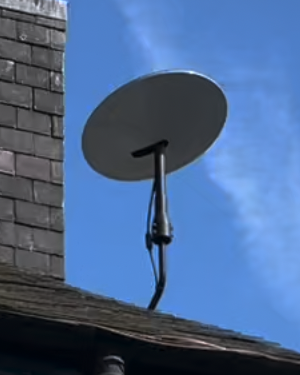
\includegraphics[width=\textwidth]{img/unstowed.png}\\\vspace{.35em}
        \centering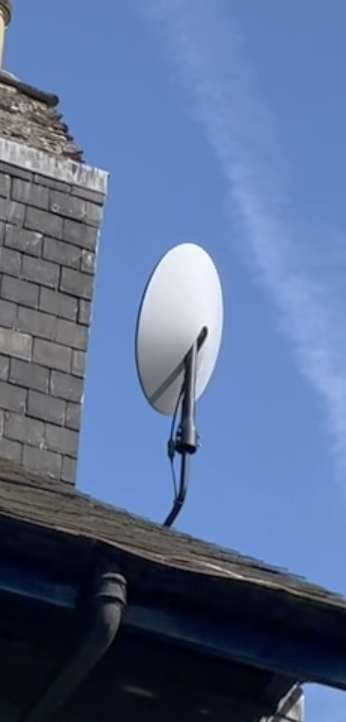
\includegraphics[width=\textwidth]{img/stowed.png}
        \caption{The dish in ``active'' and ``stowed'' modes.}
    \end{subfigure}
    \hspace{0.00005\textwidth}
    \begin{subfigure}{.4912\textwidth}
        \centering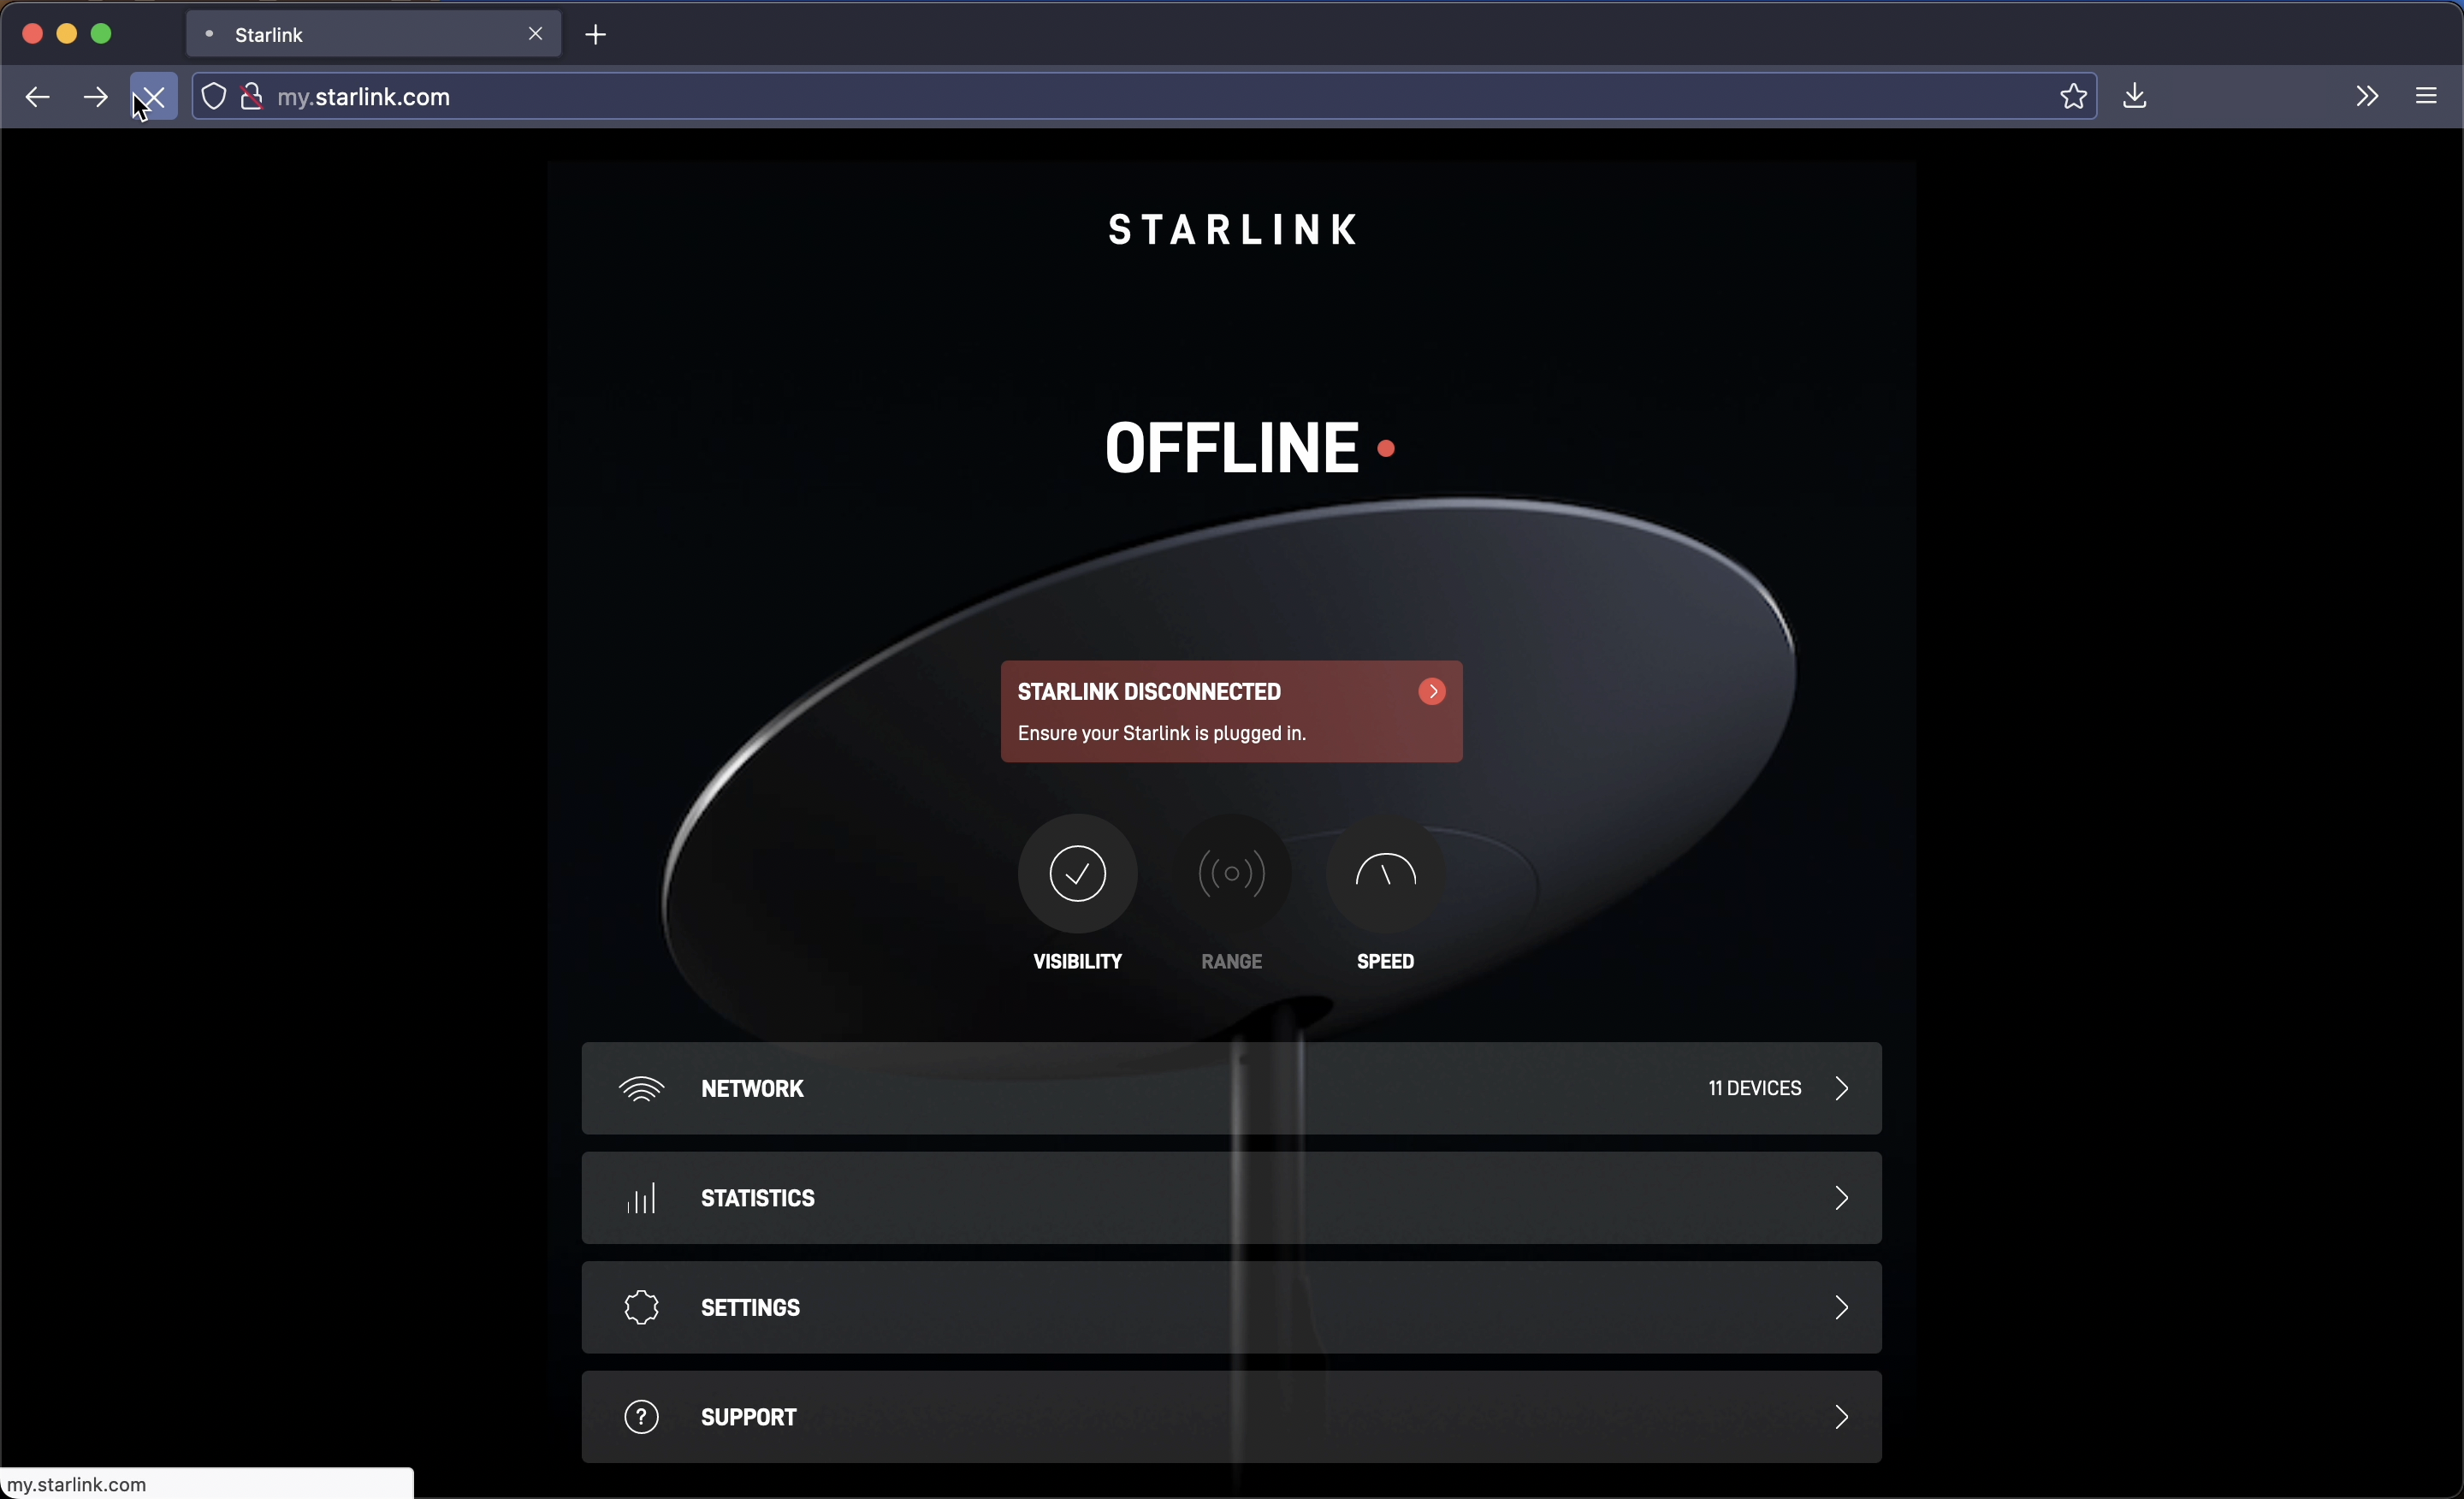
\includegraphics[width=\textwidth]{img/offline.png}\\\vspace{.35em}
        \centering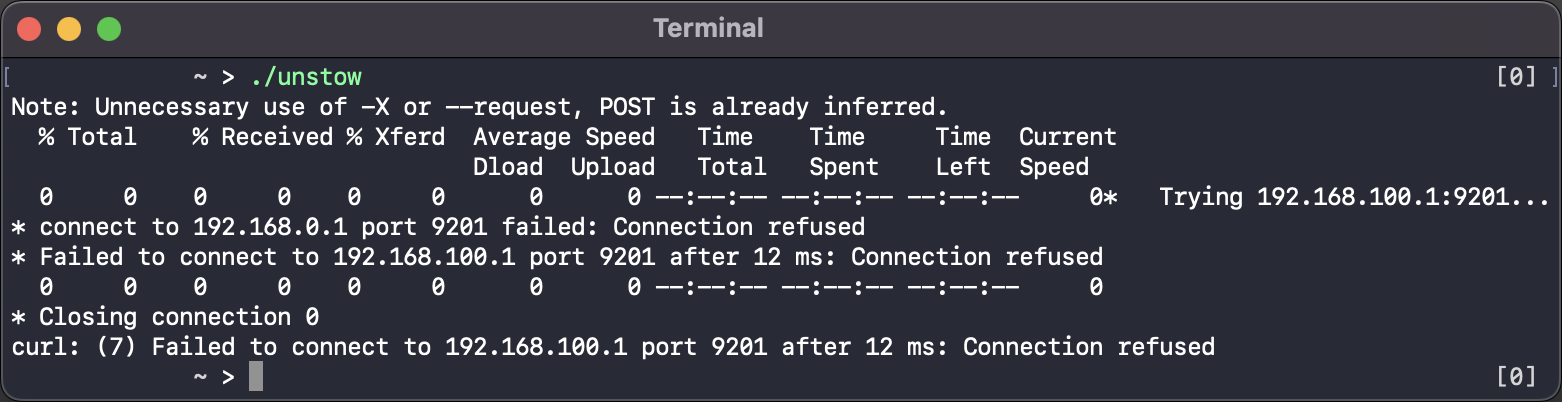
\includegraphics[width=\textwidth]{img/unstow.png}
        \caption{A screenshot of the web control panel error screen following the attack, and the result of sending commands to an inoperative dish.}
    \end{subfigure}
\vspace{-0.7em}
\caption{The outcome of a successful attack on the Starlink dish, and the resulting web control panel and response to commands.}
\label{fig:attack-outcome}
\vspace{-1.5em}
\end{figure*}

The Starlink user terminal is typically administered via the ``\url{http://my.starlink.com}'' web interface, which sends gRPC commands to the modem over the local network.
As shown in Figure~\ref{fig:modem}, these requests are decoded by a gRPC web proxy and forwarded to a command handler.

The vast majority of gRPC commands require no authentication, including commands affecting the physical state of the dish.
We note, in particular, that the ``dish stow'' command, which stops communication with the satellites, requires no authentication.

Since the gRPC payload is usually between 2 and 5 bytes, the command space can be fuzzed with random contents to discover unexpected behavior in the command handler\footnote{Source code available at \textit{\url{https://github.com/ssloxford/dishing-out-dos}}}.
Through this we discovered invalid command \lstinline{00 00 00 00 03 EA 3E 00} which causes the command handler of the user terminal to crash and no longer respond to commands.
This allows the attacker to lock the physical dish into a stowed state as seen in Figure~\ref{fig:attack-outcome}, persistently denying service even after the attacker is no longer present on the network.
Restoring internet access requires a physical power-cycle.
